\documentclass[11pt, twoside, letterpaper]{book}
\usepackage[left= 3 cm, right= 2 cm, top= 2 cm,bottom= 2 cm]{geometry}
\usepackage[spanish,active acute, es-tabla]{babel}
\usepackage{helvet}
\usepackage{sectsty}
\sectionfont{\MakeUppercase}
\subsectionfont{\MakeUppercase}
\chapterfont{\MakeUppercase}
\usepackage{multirow}
\renewcommand{\familydefault}{\sfdefault}
% add path of figures
\usepackage{graphicx,color}
\graphicspath{ {figuras/} }

\usepackage[spanish,active acute, es-tabla]{babel}
\usepackage[numbered]{bookmark}
\usepackage[final]{pdfpages}

\usepackage{apacite}
\bibliographystyle{apacite}

\usepackage{fancyhdr}
\fancyhf{}
\cfoot{\thepage}
\pagestyle{plain}


%\newlength{\bibitemsep}\setlength{\bibitemsep}{.2\baselineskip plus .05\baselineskip minus .05\baselineskip}
\newlength{\bibparskip}\setlength{\bibparskip}{11pt}
\let\oldthebibliography\thebibliography
\renewcommand\thebibliography[1]{%
  \oldthebibliography{#1}%
  \setlength{\parskip}{\bibitemsep}%
  \setlength{\itemsep}{\bibparskip}%
}

%macros 
\usepackage{fancybox}

% Abreviaciones
\newcommand{\umss}[0]{Universidad Mayor de San Sim\'{o}n}
\newcommand{\fcyt}[0]{Facultad de Ciencias y Tecnolog\'{i}a}

\newcommand{\TITULO}[0]{SISTEMA COLABORATIVO PARA EL APOYO EN EL DISE\~NO DE INTERFACES}
\newcommand{\sergio}[0]{Sergio Flores Ledezma}
\newcommand{\lic}[0]{Tutor: Maria Leticia Blanco Coca}

% Definici'on de comandos para formato

\newcommand{\comentarios}[1]{}
\newcommand{\concepto}[1]{\emph{#1}} 
\newcommand{\tips}[1]{\comentarios{#1}}
% hay que poner en el indice los conceptos


\newcommand{\linea}{\noindent \rule{12cm}{0.5mm}}

% Comentarios y notas
\newcounter{comm}
\newcommand{\parrafo}[2]{%
  \ifthenelse{\value{comm}>0}%
   {#1: \emph{#2}}%
   {}%
}
%document
\begin{document}

\frontmatter
%%%%%add the first page .pdf%%%%%%%%%%%%%%

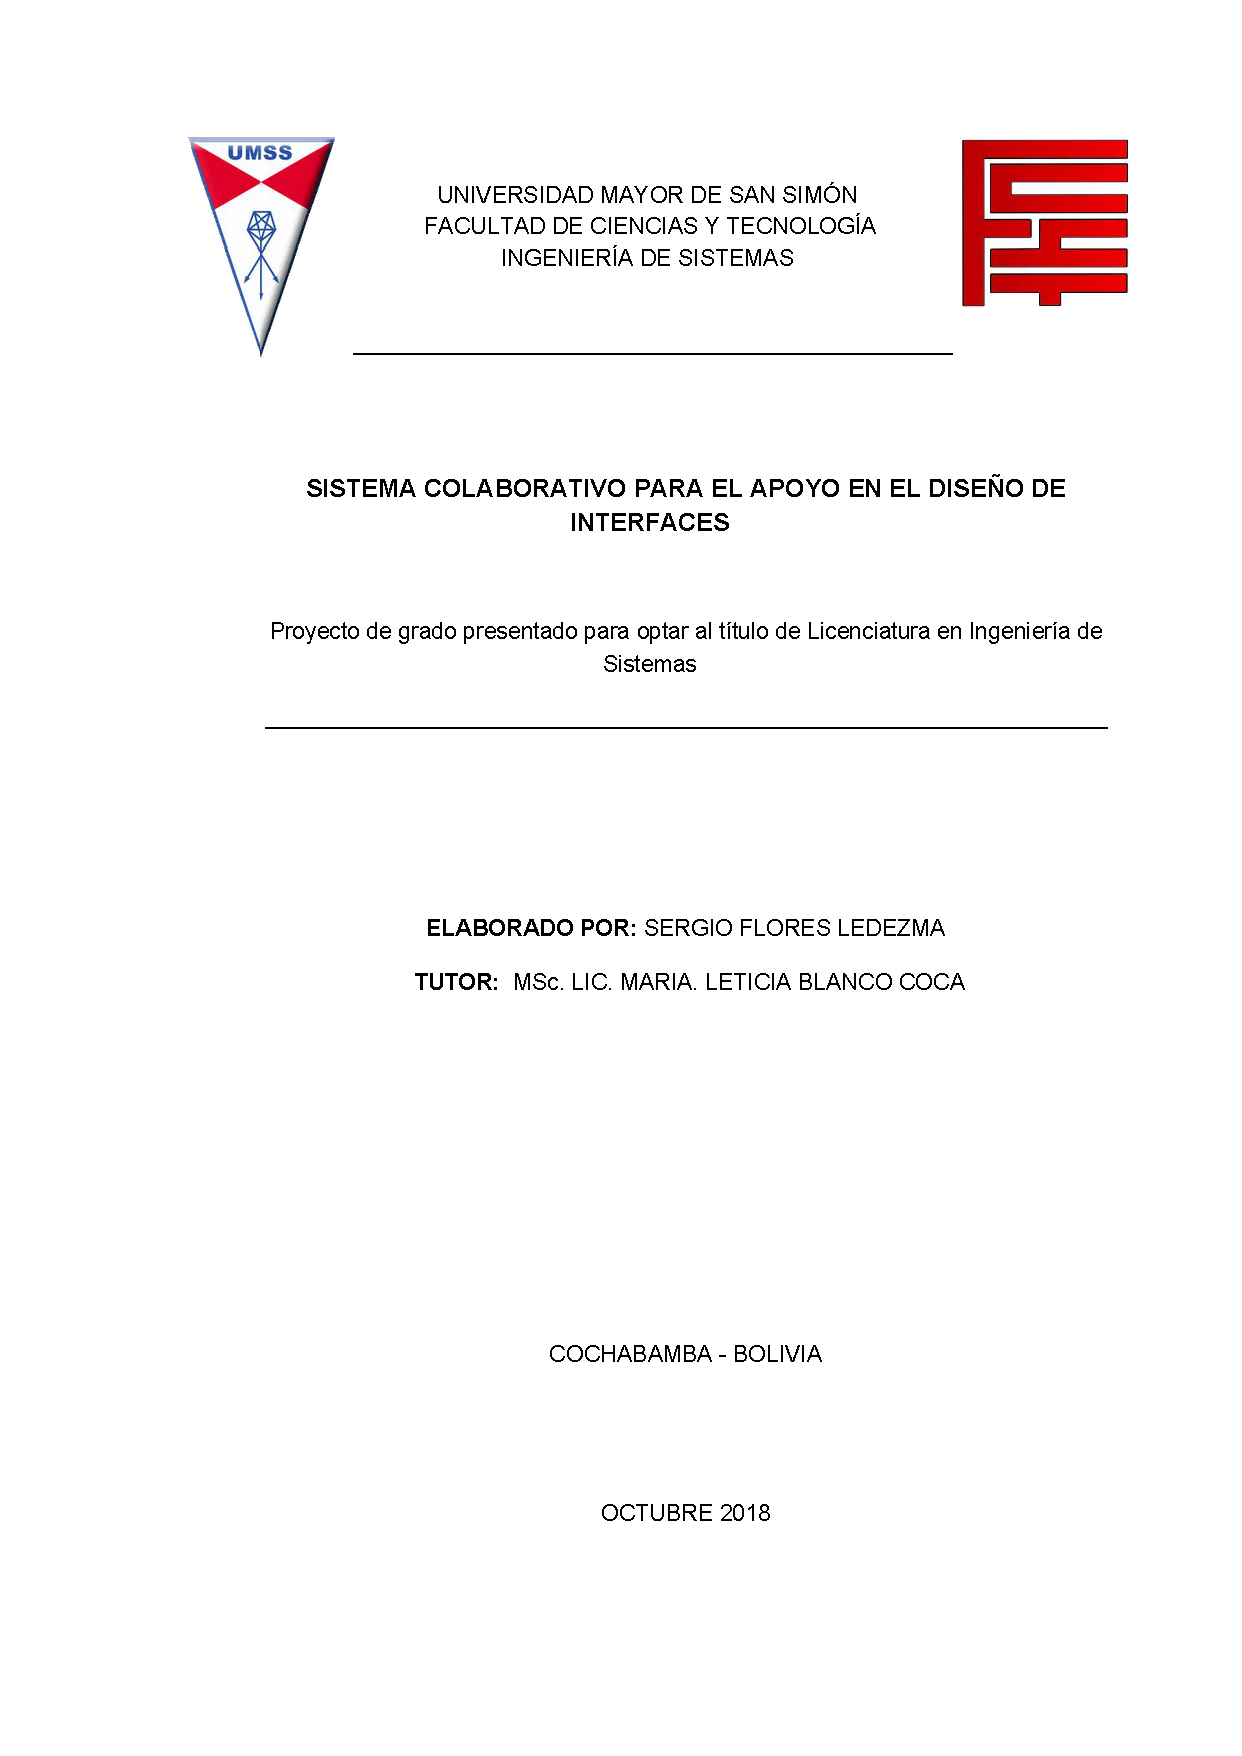
\includepdf[pages=-]{003-Caratula-Caratula.pdf}
\newpage\thispagestyle{plain}
\addcontentsline{toc}{chapter}{Dedicatoria}
\pagenumbering{Roman} % para comenzar la numeracion de paginas en numeros romanos
\label{Dedicatoria}
\vspace*{5mm}
\centerline{{\large Dedicatoria}}
\vspace{5mm}
\begin{flushright}
\textit{
Dedicado a \\
mi familia y 
a todos los que
creyeron en m'i.
}
\end{flushright}
\newpage
\clearpage\null
\newpage
\newpage\thispagestyle{plain}
\addcontentsline{toc}{chapter}{Agradecimientos}
\bookmark[page=1,level=0]{Agradecimientos}
\label{Agradecimientos}
\vspace*{5mm}
\centerline{{\large Agradecimientos}}
\vspace{2mm}
\begin{quote}

Gracias

\end{quote}
\newpage
\clearpage\null
\newpage
\newpage\thispagestyle{plain}
\addcontentsline{toc}{chapter}{Resumen}
\label{Resumen}
\begin{center}
\vspace*{5mm}{\Large \TITULO} \\

\vspace{4mm}{\large \sergio} \\

\vspace{8mm}{\Large RESUMEN}
\end{center}

\vspace{2mm}
\begin{quote}
Proximamente...
\end{quote}
\vspace{4mm}
\noindent 
\textbf{Palabras clave}: 
\emph{Colaboraci'on}, \emph{Adaptaci'on}, \emph{Conciencia}
\chapter{Lista de abreviaturas}

\begin{center}
\begin{tabular}{lcl}
UMSS   &              & Universidad Mayor de San Sim'on \\
POO    &              & Programaci'on Orientada a Objetos \\
DSL    & 			  & Domain Specific Language \\
OO     &              & Orientado a Objetos \\
IDE    &              & Integrated Development Environment \\
API    &              & Application Programming Interface \\
\end{tabular}
\end{center} %en constante avance
\newpage
\clearpage\null
\newpage
\renewcommand*{\contentsname}{Tabla de Contenido}
\tableofcontents
\renewcommand*{\listtablename}{Lista de tablas}
\listoftables\addcontentsline{toc}{chapter}{Lista de tablas}
\newpage
\renewcommand*{\listfigurename}{Lista de figuras}
\listoffigures\addcontentsline{toc}{chapter}{Lista de figuras}

\setcounter{comm}{0}

\mainmatter
\chapter{Introducci'on}
\label{capitulouno}

El dise\~no de interfaces en el 'area del desarrollo de software es una actividad muy importante, la misma es realizada por los diferentes equipos de trabajo y comprende el trabajo conjunto de un grupo de personas, lo que implica colaboraci'on y coordinaci'on al momento de realizarse.

\medskip

La participaci'on de un grupo de personas puede representar una dificultad a la hora de dise\~nar una interfaz propiamente dicha, puesto que los miembros del equipo deben generalmente hallarse geogr'aficamente en el mismo lugar y al mismo tiempo para realizar alg'un aporte inmediato, o esperar a la retroalimentacion una vez terminado el dise\~no. La mayor parte de las herramientas que ayudan en el dise\~no de interfaces son del tipo mono usuario, esto significa que solo un usuario puede usarlas a la vez.

\medskip

El proyecto pretende realizar un sistema colaborativo para coadyuvar en la coordinación de dicha actividad a partir de una herramienta ya existente, con ello se pretende facilitar la participaci'on de los integrantes del equipo permiti'endoles dise\~nar una interfaz de manera conjunta usando algunos principios de CSCW para la adaptacion de un sistema mono usuario en un sistema multiusuario.


\section{Antecedentes}

La interfaz es el medio por el cual un usuario puede interactuar con un sistema. Por ello el dise\~no de la interfaz tiende a ser fundamental dentro del desarrollo de un proyecto.

\medskip
 
Al ser esta una actividad importante se involucra una cantidad considerable de personas, como el equipo desarroll'o, el usuario para el cual est'a pensado el proyecto y algunos otros que se consideren importantes para esta actividad.

Los equipos o grupos de trabajo al involucrar cantidades determinadas de personas requieren herramientas y t'ecnicas para hacer sus tareas de la mejor forma posible y con un alto nivel de colaboraci'on.

\medskip
Se han encontrado trabajos similares como: El Sistema de Dise\~no de interfaces ``pencil'' \cite{pencil2010}
  
``\textit{Sometimes you need to see through walls – a field study of application programming interface}''. ``A veces se necesita ver a trav'ez de las paredes - un campo de estudio de aplicaciones para programar interfaces'' \cite{de2004sometimes}

\section{Definic'ion del problema}

Gran parte de los equipos de desarrollo se re'unen para tratar el dise\~no de la interfaz a ser desarrollada, lo cual conlleva a que todos los miembros del equipo se encuentren en un lugar y en un mismo tiempo lo que puede presentar un grave problema al momento de coordinar el trabajo. 

\medskip

Los sistemas de apoyo al dise\~no de interfaces en su mayor'ia son del tipo mono-usuario, lo que quiere decir que pueden ser usados por un usuario en un determinado periodo de tiempo, esto representa una limitante al momento de realizar trabajo en equipo.

Al momento de realizar el dise\~no de la interfaz los miembros del equipo pueden brindar una amplia gama de ideas, y el llevar un registro de las propuestas o los cambios realizados se torna un poco dificultoso.

\medskip

Por  lo expresado anteriormente se define el problema como:
Inadecuada coordinaci'on en el equipo para el dise\~no de interfaces lo que ocasiona dificultad en la participaci'on de los miembros del equipo de trabajo.


\section{Objetivos}

\subsection{Objetivo General}

Apoyar la coordinaci'on del equipo en el dise\~no de interfaces mediante un Sistema Colaborativo facilitando de este modo la participaci'on de los integrantes del equipo.

\subsection{Objetivos espec'ificos}

\begin{enumerate}
	\item Brindar la posibilidad de trabajo multiusuario coadyuvando al trabajo en equipo.
	\item Facilitar la retroalimentaci'on del trabajo realizado mediante un historial de acciones relevantes realizadas. 
	\item Brindar una alternativa de trabajar en un mismo proyecto desde diferentes ubicaciones.
	\item Facilitar la retroalimentaci'on de las propuestas brindadas por los miembros del equipo de trabajo.
\end{enumerate}

\section{Justificaci'on}

El proyecto se realizara tras advertir la necesidad de los equipos de desarrollo de software por fomentar la participaci'on de la mayor cantidad de personas en el dise\~no de las interfaces de un proyecto.

Se usara principios de Middleware pues es muy 'util para permitir el funcionamiento de aplicaciones distribuidas sobre plataformas heterog'eneas y homogeneas.

Se pretende tambi'en demostrar los principios de adaptacion de un sistema mono usuario a un sistema multiusuario de manera sencilla. 

\section{Alcance}

Con el proyecto brindar una herramienta capaz de permitir el trabajo de dise\~no de interfaces de usuario con la participacion de un equipo de trabajo sin la necesidad de forzar a los mismos a usar una herramienta diferente a la que estan acostumbrados.

\section{Descripci'on del contenido}

El presente proyecto fue realizado segun el flujo de trabajo presentado en las herramientas de la metodolog'ia AMENITIES
 
\chapter{Sistemas Colaborativos}
\label{capitulodos}

El trabajo en grupo es una actividad humana fundamental y los entornos colaborativos facilitan este proceso. Un aspecto crucial para su estudio y dise\~no es el uso de t'ecnicas eficientes que permitan representar los procesos de comunicaci'on, coordinaci'on y acceso a la informaci'on. Desde el nacimiento de los sistemas computacionales, el trabajo en muchos 'ambitos fue transformado dr'asticamente, con dicho cambio tambi'en surgi'o la necesidad de compartir informaci'on, recursos, memoria y otros.

\medskip
Con la aparici'on de las redes y el internet, se logr'o compartir informaci'on y algunos recursos. Pero a'un no es suficiente, puesto que tambi'en surge la necesidad del trabajo conjunto o en equipo, un claro ejemplo de dichas necesidades es el conocido caso de Linux, un sistema operativo desarrollado por gran cantidad de personas de distintas partes del mundo.
 
\medskip
Debido a la naturaleza de algunas actividades dentro el desarrollo de software, a veces es indispensable incorporar a distintos grupos de personas al momento de desarrollar alg�n trabajo espec'ifico. Dentro del dise\~no de interfaces se recomienda la incorporaci'on de diversos grupos de usuarios como ser: programadores, clientes (alg'un usuario al que va destinado el sistema), dise\~nadores gr'aficos y alg'un otro tipo de usuario que podr�a realizar aportes significativos para el dise\~no. 

\medskip
Lo descrito anteriormente denota un trabajo de colaboraci'on entre distintos tipos de personas con ideas diferentes, pero con un objetivo en com'un. Para coadyuvar en la actividad de dicho grupo, se plantea el uso de un sistema colaborativo.

\medskip
Dado que el foco del proyecto es desarrollar un sistema colaborativo, con el objetivo de identificar la utilidad del mismo dentro del proceso de creaci'on de una interfaz de usuario, es necesario plantear algunos conceptos b'asicos que  servir'an como marco conceptual y de referencia.


\section{CSCW y Sistemas Colaborativos}
Seg'un \cite{garrido2000designing} ``CSCW es una disciplina emergente que analiza el trabajo en grupo asistido por computadora, con una estrecha aplicaci'on en el control de organizaciones y distribuci'on del trabajo''. Sin embargo, este aspecto cada vez tiene un sentido m'as amplio, lo que permite recoger entornos en los cuales se produce interacci'on entre participantes con diversos fines (educativos, visitas tur'isticas, ocio, etc.), con diferentes habilidades de los usuarios implicados, distintos medios y soportes de acceso (computaci'on ubicua). 
El t'ermino ``Computer-supported Cooperative Work (CSCW)'' introducido por Irene Greif y Paul M.Cashman
\cite{brown1985interfaces} se refiere a ``C'omo las actividades colaborativas y su coordinaci'on pueden ser apoyadas por medio de sistemas computacionales.'', CSCW suele ser interpretado como un sin'onimo de sistema colaborativo, sin embargo algunos autores afirman que, mientras los sistemas colaborativos se refieren a sistemas computacionales reales, CSCW se enfoca en estudiar las herramientas y las t'ecnicas de un sistema colaborativo as'i como su impacto psicol'ogico, social y el efecto organizacional que causa. Wilson \cite{wilson1991computer} define los CSCW de la siguiente manera:

\medskip
\emph{``CSCW es un t'ermino gen'erico, que combina la comprensi'on de la forma en que las personas trabajan en grupo usando tecnolog'ias de redes de computadoras y hardware asociado, software, servicios y t'ecnicas.''}
\medskip

En cambio define los Sistemas colaborativos  como:

\medskip	
	\emph{``Actividades de grupo intencionales con software para su apoyo.''}
\medskip	

Dentro del software colaborativo se puede encontrar: los Groupware y Workflow que son las tecnolog'ias m'as usadas y que ser'an brevemente descritas a continuaci'on.

\subsection{Groupware}
La relaci'on usuario m'aquina comenz'o a cambiar a medida que el software fue evolucionando, un claro ejemplo se present'o en software orientado al entretenimiento (videojuegos), que a medida que los usuarios comenzaron a necesitar algo m'as que un mero pasatiempo, se comenz'o a desarrollar caracter'isticas importantes como el soporte a multijugador en l'inea, el cual permite a varios usuarios encontrarse en el mismo videojuego. En muchas labores dentro del 'ambito empresarial se necesita interactuar con grupos de personas, en este contexto trasladar la caracter'istica de esos videojuegos antes mencionada puede ser muy 'util, el interactuar con las personas que necesitas en tiempo real sin necesidad de tenerlos en el mismo lugar geogr'afico, lo cual  representa una gran ventaja al momento de realizar ciertas actividades.
 
 \medskip
Los groupware \cite{ellis1991groupware} son un tipo de sistemas colaborativos que se enfocan en ayudar a los equipos de trabajo a realizar actividades mediante una red. Para describir un Groupware tomaremos la siguiente definici'on:

\medskip 
\emph{``Sistemas basados en computadoras que apoyan a grupos de personas que trabajan en una tarea com'un y que proveen una interfaz para un ambiente compartido'' -Dave Chaffney }
\medskip

Los Groupware hacen 'enfasis en tres caracter'isticas muy importantes: ``Colaboraci'on, Comunicaci'on y Coordinaci'on''  \cite{ellis1991groupware}. Estos tres elementos son fundamentales a la hora de trabajar en equipo. A su vez buscan promover un ambiente compartido de colaboraci'on, en el que se perciba realmente el trabajo en equipo, un ambiente en el que se pueda interactuar con las dem'as personas no solo en el trabajo desempe\~nado, sino tambi'en mediante texto, voz o video.

\medskip
Se puede notar en la definici'on de Groupware que esta no define que el trabajo deba que ser simult'aneo. Estos sistemas pueden proveer diferentes tipos de soporte de acuerdo a las necesidades que se presenten; Si el trabajo dentro del Groupware es efectuado por los usuarios al mismo tiempo, se lo define como s'incrono, de lo contrario, si el trabajo es efectuado en distintos lapsos de tiempo por los usuarios, es definido como as'incrono. Si el trabajo se realiza desde diferentes lugares geogr'aficos se denomina distribuido; esto puede verse de mejor manera en la siguiente figura \ref{fig:GroupWareTimeMatrix}:

\begin{figure}[ht]
\centering
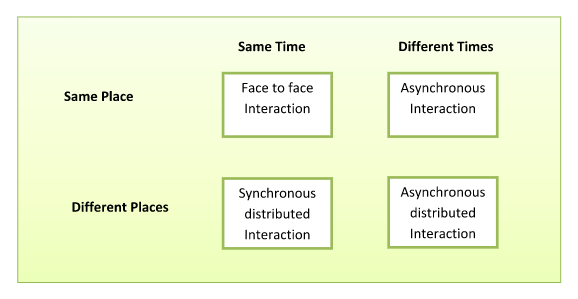
\includegraphics[width=0.75\textwidth]{Figura0201GroupWareTimeMatrix}
\caption{Groupware Time Space Matrix. Fuente:}
\cite{ellis1991groupware}
\label{fig:GroupWareTimeMatrix}
\end{figure}
\medskip

CSCW se convirti'o en un campo de investigaci'on amplio que abarca desde el an'alisis sociol'ogico sobre la forma de trabajar en grupos a las tecnolog'ias inform'aticas que apoyan el trabajo en grupo de las personas. 

\medskip
Existe una delgada l'inea que separa a los sistemas que son considerados groupware y los que no. El criterio m'as importante \cite{ellis1991groupware} para poder definir un groupware es el soporte que ofrece al trabajo en equipo, por ejemplo un sistema que brinda soporte al trabajo de m'ultiples usuarios, pero en 'areas diferentes y realizando tareas diferentes tiene un bajo nivel de cooperaci'on, a diferencia de un sistema pensado para dar soporte a m'ultiples usuarios realizando una tarea conjunta en un espacio compartido, por ejemplo el caso de google docs.
El desarrollo de software es una actividad donde el trabajar de manera distribuida es algo que sucede regularmente, se tienen varios ejemplos grandes de dicha situaci'on como ser el conocido caso del sistema operativo Linux.

\medskip
Entre los criterios que se toman para catalogar un groupware como tal, est'an el desarrollar la misma tarea y el estar presentes en espacio compartido. Por ejemplo, un sistema de tiempo compartido permite que m'ultiples usuarios realicen actividades, pero estos pueden tener metas diferentes, por lo tanto realizar'an tareas diferentes, en cambio un sistema que permite editar un documento de manera conjunta (google docs), est'a enfocado a que los usuarios que ingresen al sistema tengan en mente una misma meta, lo cual se refleja en las actividades que se realicen. De igual forma un sistema de mensajer'ia permite que dos usuarios puedan interactuar y enfocarse en una misma tarea, pero el ambiente y la colaboraci'on no son muy notorios, en cambio el sistema que permite el dise\~no de la interface tiene que dar soporte para que los usuarios puedan percibir lo que sus compa\~neros est'an haciendo.

\subsection{Workflow}

\medskip
Los Workflows son sistemas que ayudan a administrar y automatizar procesos de negocios en los que participan diferentes usuarios.

La WfMC (Workflow Management Coalition) define a los Workflows Como:

\medskip 
\emph{``La automatizaci'on de un proceso de negocio, total o parcial, en la cual documentos, informaci'on o tareas son pasadas de un participante a otro a los efectos de su procesamiento, de acuerdo a un conjunto de reglas establecidas.''}
\medskip

En la misma definici'on radica la diferencia entre groupware y workflow, dado que los groupware son sistemas orientados al trabajo conjunto, en cambio los workflow est'an orientados dar soporte al conjunto de personas que realizan distintas tareas siguiendo un flujo de trabajo. Debido a los diferentes tipos de procesos que se pueden dar soporte con un workflow se definen:

\medskip 
a) Workflows de Producci'on: o tambi'en llamados Workflows de transacciones; las transacciones son la base de las acciones dentro de las bases de datos, los workflow de producci'on en general automatizan procesos de negocios que tienden a ser repetitivos y con gran manejo de datos.

\medskip
b) Workflows de Colaboraci'on: Los workflow que est'an orientados a resolver procesos de negocios donde participan grupos de personas que tienen una meta com'un son denominados Workflows de colaboraci'on.

\medskip
c) Workflows de Administraci'on: Son aquellos que est'an orientados a dar soporte a la los procesos de administraci'on de una empresa o negocio.
\medskip

Se puede afirmar que los Workflow son herramientas muy 'utiles para identificar y evaluar procesos, tambi'en son muy importantes al hacer un trabajo de reingenier'ia puesto que su principal enfoque es el integrar a las personas y los procesos que se llevan a cabo dentro de un negocio.

\medskip
Despu'es de haber definido la diferencia entre groupware and workflow y tomando en cuenta las caracter'isticas que ambas opciones presentan, se opt'o por los Groupware como el centro te'orico del presente proyecto, dadas las facilidades en el apoyo a la colaboraci'on dentro de un trabajo grupal, que es exactamente lo que se busca al momento de dise\~nar interfaces de usuario.


\section{Awareness}
En un WYSIWIS (What you see is what I see- Lo que ves es lo que veo) relajado, los usuarios pueden trabajar en diferentes partes de un espacio compartido. En dicha circunstancia es importante que el usuario sea consciente del estado de los otros usuarios, para que de esa manera pueda colaborar de manera natural y fluida con ellos. En este 'ambito se habla de la conciencia de grupo (awareness) tambi'en definida como momento de comprensi'on de la interacci'on de otra persona con el espacio compartido. \cite{gutwin1996workspace}

\medskip
El awareness es fundamental en los sistemas colaborativos, puesto que incrementa significativamente la usabilidad del sistema \cite{gutwin1996workspace}. Es usado principalmente para, simplificar la comunicaci'on, coordinar acciones, ayudar a los usuarios a anticipar futuras acciones y entender la ayuda de los dem'as. \cite{gutwin1996workspace}, la informaci'on de la conciencia de grupo consiste en los diferentes elementos listados en la siguiente figura \ref{fig:WorkspaceAwareness}.

\begin{figure}[ht]
    \centering
    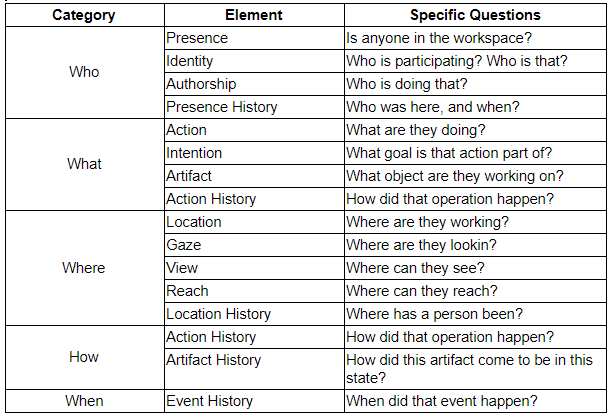
\includegraphics[width=0.75\textwidth]{Figura0202WorkspaceAwareness}
    \caption{Composition of workspace awareness information. Fuente: Grudin and Greenberg 2002}
    \label{fig:WorkspaceAwareness}
\end{figure}
\medskip

La primera columna de la tabla lista b'asicamente las categor'ias de la informaci'on del awareness, incluyendo: con quien estamos trabajando, que es lo que est'an haciendo, donde estan, como estan ocurriendo dichos eventos, cuando estos eventos est'an sucediendo. 

\medskip
En cada categor'ia existen diferentes elementos de conciencia, cada elemento describe una respuesta a cada pregunta que se puede realizar dentro de un espacio compartido las cuales se muestran en la tercera columna. (Gutwin and Greenberg 2002). 

\medskip
Para llenar la informaci'on requerida en el awareness, existen diferentes herramientas que son usadas com�nmente por los sistemas colaborativos:

\medskip
Telepointer: El telepointer es la manifestaci'on del puntero remoto de otro usuario, que se muestra en el sistema del usuario local.

\medskip
Multi-user Scrollbar: el multi-user scrollbar es una extensi'on del scrollbar simple, que indica la posici'on de los dem'as usuarios.

\medskip
Radar view: el radar view es una herramienta para entregar una informaci�n m'as detallada de la ubicaci'on de un usuario, se usa generalmente cuando el sistema colaborativo presenta m'as de un espacio compartido para el trabajo.

\medskip
En adici'on a las herramientas descritas existen otras no tan frecuentes que pueden ser de gran ayuda de acuerdo a las caracter�sticas del sistema en cuesti'on, dichas herramientas pueden ser el sonido, una lista de usuarios con la informaci'on de su sesi'on, video, areas de intercambio de mensajes, entre otros.


\section{AMENITIES: Metodolog'ia para el estudio y desarrollo de sistemas cooperativos}
Cuando se realiza alg'un proceso que implica la colaboraci'on entre personas, lo primero que se debe tener en cuenta es la estructura y la organizaci�n de dicho grupo de trabajo. Como resultado se tienen como tareas fundamentales el recoger los aspectos organizativos, cognitivos y de interacci�n que representen de manera adecuada las demandas del trabajo en concreto.

Existen propuestas dentro del dise\~no de sistemas colaborativos que ofrecen notaciones con diferente nivel de formalismo y abstracci'on para recoger aspectos relativos a dichos sistemas. Dentro de la amplia gama de propuestas se encuentran GTA [welie] y ConcurTaskTrees [Paterno,97]. La primera se centra en la descomposici'on de tareas y asignaci�n de actividades a roles, en cambio CTT se centra m'as en aspectos de coordinaci'an ( uso temporal de espacios comunes), sin embargo estas propuestas no dejan de ser parciales y no cubren las caracter�sticas de los sistemas colaborativos, a su vez son dif'iciles de enlazar con tecnicas de Ingenieria de Software.

Para trabajar sobre la complejidad inherente a los entornos colaborativos, se ha propuesto el uso de una metodolog'ia conocida como ``AMENITIES'', que permite describir un sistema colaborativo mediante cuatro vistas que facilitan detectar los aspectos m'as relevantes de los sistemas de este tipo.

AMENITIES (acr'onimo de A Methodology for aNalysis and DesIgn of CooperaTIve systEmS) [Garrido, 03] integra de modo jerarquizado varios modelos de comportamiento y tareas, con la idea de proporcionar una representaci'on del sistema colaborativos en su conjunto y con diferentes vistas complementarias. 


\subsection{Vista de grupo}

Para la vista de grupo, primeramente se debe identificar los aspectos propios del grupo u organizaci'on, y las restricciones que se imponen. Dichas organizaciones se articulan bajo ``roles'', que determinan las relaciones entre los miembros del grupo y las tareas que est'an bajo su cargo. 

Las relaciones, normalmente est'an condicionadas por una serie de restricciones impuestas al sistema colaborativo, y se pueden identificar como m'as importantes las siguientes:

\begin{itemize}
	\item Capacidades: Son restricciones cognitivas que se imponen a cada actor para participar en un rol determinado. Estas capacidades determinan los conocimientos que se debe adquirir por un usuario para participar en un rol concreto.
    \item Leyes: Son restricciones impuestas por la organizaci'on e identifica las reglas que se deben preservar en un grupo. Normalmente estas reglas son la misma estructura social que se manifiesta en el grupo(jerarqu'ia, democracia, etc.)
\end{itemize}

Ambas restricciones permiten modelar sistemas din'amicos, es habitual que tanto la estructura del grupo como su funcionamiento se modifique en el tiempo (los participantes pueden adquirir nuevas capacidades, variar en n'umero de miembros que lo conforman o bien, modificar las leyes que rigen el grupo al aplicar nuevas estrategias de trabajo). 


\subsection{Vista de cognitiva}
La vista cognitiva representa el conocimiento que posee o adquiere cada miembro del grupo en el escenario colaborativo. Este conocimiento queda reflejado mediante la descripci'on de las tareas que puede llevar a cabo.

La descripci'on de las tareas implica un an'alisis profundo de las actividades que se deben realizar en el grupo, la divisi'on del trabajo y determinar las interrelaciones que existen entre ellas. El an'alisis de tareas contempla todos estos pasos, y las divide en dos fases claramente diferenciadas. 

En primer lugar se define la denominada interfaz del rol, que recoge las caracter'isticas m'as relevantes de las tareas a desempe\~nar por un rol junto a las interrelaciones con el resto de participantes (tareas) y entorno (mediante eventos).
 
Los aspectos m'as relevantes que identificamos en el interfaz del rol son:

\begin{itemize}
	\item Identificar tareas a desempe\~nar
	\item Relaci'on con otras tareas tales como:
	\begin{itemize} 
		\item Si puede ser interrumpida por otra tarea 
		\item Su naturaleza cooperativa 
		\item Mecanismo de activaci'on y modos de sincronizaci'on 
	\end{itemize}
\end{itemize}

\medskip

Este tipo de relaciones modelan el comportamiento tanto del usuario como del propio entorno. Las mismas se modelan mediante eventos que provocan cambios en el entorno (y en las pol'iticas que determinan el comportamiento del sistema). 

\medskip

En la segunda fase, se describe y pormenoriza cada tarea mediante una descomposici'on jer'arquica, que se completa con informaci'on y aspectos recogidos de otras vistas. En esta descripci'on de tareas usaremos notaciones que nos permite especificar secuencialidad, concurrencia, optatividad, decisiones, etc.

\medskip
Posteriormente, se detalla las tareas tanto individuales como cooperativas, y en las cuales, puede aparece informaci�n relativa a otras vistas.

\subsection{Vista de interacci'on}
La vista de interacci�n abarca otros aspectos que se deben estudiar como ser los procesos que implican un di�logo entre participantes para analizar sus caracter�sticas, concretamente: 

\begin{itemize}
	\item El modo de di�logo que se producen entre participantes 
	\item Los requisitos que impone ese di�logo sobre los medios a utilizar
\end{itemize}

\medskip
Este modo de di�logo se identifica mediante protocolos. Los protocolos se pueden analizar por separado dentro de la organizaci�n ya que en gran medida son independientes del dominio del problema, y por tanto, se pueden incorporar al an�lisis de tareas. Por ejemplo, se pueden identificar protocolos democr�ticos (toma de una decisi�n por mayor�a), consenso (aprobaci�n un�nime de una decisi�n), jer�rquica, etc.

\subsection{Vista de informaci'on}

En la vista de informaci'on, se debe recoger la informaci'on que es compartida en el escenario. Esta informaci'on se puede describir de manera impl'icita en las actividades y acciones o bien, de modo expl'icito como flujo de informaci'on entre actividades. La informaci'on que fluye a trav'es del sistema colaborativo ser'an los documentos (los objetos que son gestionados en el sistema), eventos y recursos. 

\section{Refactorizaci'on}

AMENITIES est'a centrada en el modelado inicial del sistema usando el punto de vista del usuario y teniendo muy en cuenta aspectos relacionados con el grupo (conciencia de grupo, relaciones entre usuarios, din'amica del grupo, representaci'on de aspectos sociales, etc), dicha definici'on permite la posibilidad del desarrollo de un sistema colaborativo ya sea desde su inicio, o transform'andolo a partir de un sistema ya realizado, agregando las caracter'isticas ya mencionadas, puesto que la din'amica de grupo representa la evoluci'on del contexto en el que se va a realizar la colaboraci'on entre los usuarios.

\medskip
Durante el desarrollo de sistemas colaborativos, existen dos opciones, la creaci'on de un sistema colaborativo o refactorizar una aplicaci'on mono-usuario en una aplicaci'on multi-usuario [Qian Xia, 06], para realizar la refactorizaci'on se debe tomar en cuenta los siguientes requerimientos:

\begin{itemize}
	\item Compatibilidad de la Aplicaci'on: Las caracter'isticas de la interfaz, funcionalidades y formatos de la aplicaci'on mono-usuario original deben mantenerse.

	\item Transparencia de la aplicaci'on: no deben realizarse cambios en el c'odigo fuente original.

	\item Respuesta local r'apida: la interacci�n con el sistema en un medio local debe ser tan r'apida como la respuesta del sistema original.

	\item Colaboraci'on sin restricci'on: Se debe permitir a los usuarios cualquier operaci'on sobre objetos de datos en cualquier momento, lo que implica un WYSIWIS (What you see is what i see) relajado y trabajo simultaneo.
	\item Workspace Awareness: El sistema debe soportar una variedad de caracter'isticas relacionadas a la conciencia de grupo dentro de los espacios de trabajo, de tal manera el usuario puede saber quien esta en su grupo de trabajo, donde se est'a trabajando y que es lo que se est'a trabajando.

	\item Administraci'on de sesi'on: El sistema debe proveer una administraci'on de sesi'on ligera y flexible, para soportar que usuarios administran el trabajo con poco esfuerzo.

	\item Control de interacci'on flexible: El sistema debe proporcionar una variedad de control de interacci'on paradigmas / pol'iticas que van desde la interacci'on simult'anea y libre, hasta la interacci'on secuencial y sincronizada con el fin de facilitar la eficacia de diferentes tareas de colaboraci'on.

\end{itemize}

\medskip
Debido a que la refactorizaci'on de un sistema puede llegar a tornarse bastante compleja, existen trabajos previos que sirven como marco de referencia para futuros trabajos, tal es el caso de CoWord y CoPowerPoint aplicaciones colaborativas realizadas a partir de Word y PowerPoint respectivamente [Qian Xia, 06].

\subsection{Arquitectura centralizada y replicada}

Al momento de realizar un sistema colaborativo, se debe escoger la arquitectura que soporta la aplicaci�n, la arquitectura de los sistemas colaborativos puede ser clasificada en dos grupos, la arquitectura centralizada y la arquitectura replicada (Lauwers, 90).

\medskip
Con la arquitectura centralizada, existe 'unicamente una instancia de la aplicaci'on compartida ubicada en un sitio central. Los dem'as sitios colaborativos cuentan simplemente con sistemas clientes que cuentan con funciones limitadas de acuerdo al rol que desempe\~nan dentro del plan de trabajo. El cliente b'asicamente dispara eventos para la aplicaci�n compartida, dichos eventos generan informaci'on en el sistema central de la aplicaci'on, la cual luego es distribuida y mostrada en el o los sistemas cliente.

\begin{figure}[ht]
    \centering
    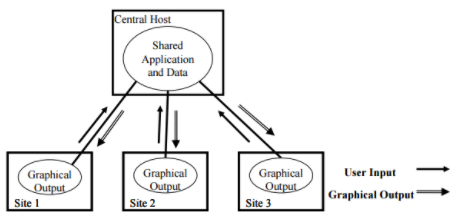
\includegraphics[width=0.75\textwidth]{Figura0203ArquitecturaCentralizada}
    \caption{Arquitectura centralizada. Fuente: Lauwers 90 }
    \label{fig:ArquitecturaCentralizada}
\end{figure}
\medskip

La principal ventaja de la arquitectura centralizada es su facilidad de implementaci'on a comparaci'on de la arquitectura replicada puesto que solamente se tiene que mantener una instancia de la aplicaci'on compartida, los desarrolladores no tienen que poner mucha energ'ia en la consistencia de la informaci'on. Pero la centralizaci�n tambi'en presenta desventajas, la m'as significativa es la lentitud en la respuesta local, cada evento local debe ser enviado a la aplicaci'on compartida, la vista local no puede ser actualizada hasta que la informaci'on sea recibida correctamente en la aplicaci'on central. La espera puede tornarse muy alta mientras mayor sea el retardo de la red. 

\medskip
Dichos problemas motivaron la arquitectura replicada, en la que cada uno de los sitios colaboradores tiene una instancia de la aplicaci'on compartida, corriendo en el sitio local. La arquitectura replicada es capaz de realizar una respuesta r'apida gracias a que los eventos disparados por el usuario pueden ser ejecutados de manera local antes de ser enviados a los sitios remotos. 

\begin{figure}[ht]
    \centering
    \includegraphics[width=0.75\textwidth]{Figura0204ArquitecturaReplicada}
    \caption{Arquitectura replicada. Fuente: Lauwers 90 }
    \label{fig:ArquitecturaReplicada}
\end{figure}
\medskip

De cualquier manera la arquitectura replicada tambi'en presenta problemas, el m'as significativo es mantener la consistencia. Si se permite a los usuarios interactuar con su aplicaci'on local y replicar libremente, los eventos pueden ser ejecutados en diferente orden en los distintos sitios distribuidos. Sin embargo la arquitectura replicada facilita el WYSIWIS y tambi'en elimina el retardo en el tiempo de respuesta de la aplicaci'on.


%(8-10pp)
\chapter{Interfaces De Usuario}
\label{capitulotres}

Dentro de este cap'itulo se hablar'a sobre algunas caracter'isticas importantes que se tienen que tomar en cuenta para el dise\~no de interfaces de usuario y algunas t'ecnicas que se utilizan para fundamentar el desarrollo del trabajo de grado.

\section{Interfaz De Usuario}
Se puede definir a la interfaz de usuario como el elemento encargado de permitir la comunicaci'on del usuario con la m'aquina o el sistema. Dada esta definici'on, necesitamos describir dos elementos importantes para poder entender mejor a una interfaz de usuario:

\begin{itemize}
	\item Elementos de entrada: Elementos  de informaci'on ingresados por el usuario, como ser: 'ordenes, comandos o cualquier otro elemento que el usuario pueda ingresar como pauta de lo que quiere conseguir.

	\item Elementos de salida: Son los elementos obtenidos de las acciones ejecutadas por el usuario, que acercan al mismo a obtener lo que espera y lograr así su meta.
\end{itemize}

\medskip
Las interfaces de usuario se pueden clasificar en tres tipos: F'isicas, Gr'aficas, y Tangibles. Los cuales son descritos brevemente a continuaci'on.

\begin{itemize}
	\item \textbf{PUI (\textit{Physical User Interface} - Interfaz de usuario f'isica):} Son las interfaces de usuario f'isicas, generalmente presentes en maquinaria, autos, u otros, son los medios mec'anicos mediante los cuales un usuario puede comunicarse con un sistema determinado.
 
	\item \textbf{ GUI (\textit{Graphical User Interface} - Interfaz de usuario gr'afica):} Son las interfaces gr'aficas generalmente presentes en sistemas computacionales o sistemas digitales, constan de elementos gr'aficos (botones, texto, im'agenes, etc.) dentro de una pantalla en el computador.

	\item \textbf{TUI (\textit{Tangible User Interface} - Interfaz de usuario tangible):} Las Interfaces de usuario tangibles emplean objetos reales para representaci'on y control en un medio computacional. Este tipo de interfaz de usuario est'a presente generalmente en sistemas de entrenamiento o simulaci'on, donde por ciertos motivos no se puede interactuar con un sistema real pero se intenta que la experiencia del usuario sea lo m'as parecida a ella.
\end{itemize}

\medskip
Las GUI han ido evolucionando de la mano de la tecnolog'ia, podemos ver claramente esto en su historia, cuando se pas'o de un texto plano siendo ejecutado como 'ordenes al computador, a un elemento visual orientado a satisfacer distintos tipos de necesidades de los usuario. Con la evoluci'on tambi'en se generaron criterios que nos permiten diferenciar la calidad de las GUI, permitiendo de esta manera un mayor desarrollo y aprovechamiento de este elemento tan importante.
Entre dichos criterios sobresalen enormemente dos, que son: la usabilidad  y la naturalidad.

\subsection{Usabilidad}
La usabilidad, es una caracter'istica muy importante para obtener la aprobaci'on del usuario en cualquier sistema, la misma se define como el elemento que mide el grado en el que el usuario puede realizar sus actividades, mientras más sencillo le resulte al usuario realizar sus actividades m'as usable ser'a la interfaz, por ende m'as usable ser'a el sistema. 
La usabilidad abarca dos conceptos fundamentales:

\begin{itemize}
	\item \textbf{Funcionalidad:} Que se refiere a las caracter'isticas del sistema que permiten al usuario realizar sus tareas.

	\item \textbf{Facilidad de uso:} Se provee caracter'isticas para que el sistema sea más f'acil de aprender y permite realizar tareas m'as f'acilmente.

\end{itemize}

\medskip
Cuando se usa el t'ermino usabilidad los programadores se enfocan especialmente en el primer concepto, dejando de lado factores esenciales como la experiencia del usuario cuando intenta usar el sistema, se olvida preguntarse, ¿el usuario puede encontrar lo que busca?, ¿El sistema le permite realizar su trabajo m'as f'acil?
Se puede decir que la usabilidad consiste de seis factores los cuales son presentados a continuaci'on:

\begin{itemize}
	\item \textbf{ Apto para el uso (Funcionalidad): } El sistema soporta las tareas que tienen los usuarios en la vida real.
	
	\item \textbf{F'acil de Aprender:} El sistema es f'acil de usar para distintos grupos de usuarios.

	\item \textbf{Eficiencia en las Tareas:} Cuan eficiente es el sistema para los usuarios frecuentes.

	\item \textbf{F'acil de Recordar:} Cuan f'acil de recordar es para los usuarios ocasionales.

	\item \textbf{Satisfacci'on Subjetiva:} Cu'an satisfecho est'a el usuario con el sistema.
	
	\item \textbf{Entendible:} Cu'an f'acil es entender lo que el sistema est'a haciendo. Este factor es muy importante en ciertas ocasiones como ser fallas del sistema o errores.
\end{itemize}

\medskip

\subsection{Naturalidad}
La naturalidad es una caracter'istica que se enfoca m'as a cu'an natural es para el usuario realizar sus actividades, por ejemplo los usuarios en general est'an acostumbrados a salir de los programas mediante un bot'on en una de las esquinas superiores de la ventana, dicho bot'on est'a representado por una x, cambiar esto podr'ia significar un choque con lo que el usuario conoce, esto le restar'ia naturalidad a la interface que se est'a desarrollando, por lo tanto lo que se intenta con esta caracter'istica es presentarle al usuario elementos que ya conoce para poder estimular su memoria y facilitar su trabajo, pues se dice que la memoria es la forma m'as simple de inteligencia.
Dadas las anteriores definiciones podemos continuar describiendo el proceso de dise\~no de una interfaz de usuario con algunas heur'isticas para lograr un mejor resultado.

\section{Dise\~no de interfaces gr'aficas de usuario}
Soren Lauesen \cite{lauesen2005user} sostiene que, si consultamos a un programador sobre la interfaz de usuario, el responde que es un elemento sencillo, que se puede realizar despu'es de haber concluido las tareas m'as importantes del sistema, en cambio si trasladamos la misma pregunta al dise\~nador de interfaces, este nos dice que es uno de los elementos m'as importantes dentro del desarrollo de un proyecto, y que por ende debe realizarse antes que las dem'as tareas, y en participaci'on con programadores, clientes, dise\~nadores y otros.
Podemos evidenciar que se tienen puntos de vista diferentes, y se puede afirmar que ambos tienen algo de raz'on, hacer una interfaz de usuario es una tarea relativamente sencilla, pero hacer una interfaz de usuario que agrade al cliente es ya una tarea mucho m'as complicada.
Existen diversas t'ecnicas que pueden ser usadas dentro del dise\~no de interfaces una de las m'as importantes y la que se tratara a lo largo de este art'iculo es el sketch (prototipado) y sus ventajas.

\subsection{Sketch Design}

Sketch es una t'ecnica de dise\~no muy ventajosa en diversos aspectos, este m'etodo de dise\~no se basa esencialmente en el prototipado.
	El prototipado es una pr'actica muy usada en el 'ambito de la arquitectura, por el costo que implica no se puede realizar pruebas reales en las que las personas puedan caminar, as'i que se realizan modelos en papel, maquetas, planos, etc. Para permitir que el o los usuarios puedan opinar sobre el producto antes de que  el mismo est'e terminado, esta pr'actica es muy 'util a la hora de ahorrar tiempo y dinero. El sketch modeling se basa en desarrollar modelos mediante dibujos de la interfaz de usuario.
¿Por qu'e realizar prototipos?
Los prototipos son f'aciles y r'apidos de desarrollar, f'aciles de cambiar y f'aciles de desechar, permite ahorrar tiempo y dinero, permite contar con diferentes alternativas, solucionar problemas antes de que el c'odigo sea escrito y mantener el enfoque del dise\~no en el usuario.
El prototipado de una interfaz de gr'afica puede tener diversos tipos de fidelidad, la fidelidad de un prototipo se mide de acuerdo al nivel de detalle que se us'o al momento de realizar el prototipo, existen 3 niveles de fidelidad: low fidelity, m'edium fidelity, high fidelity. 

\begin{itemize}
	\item \textbf{Low Fidelity}
	Son los prototipos de fidelidad baja, que son llamados trazos art'isticos, el prototipo est'a formado por dibujos simples y de baja representaci'on, como se muestra en la siguiente figura \ref{fig:LowFidelity}.

\begin{figure}[ht]
    \centering
    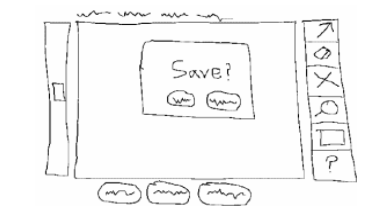
\includegraphics[width=0.75\textwidth]{Figura0301LowFidelity}
    \caption{Ejemplo de un prototipo de baja fidelidad.}
    \label{fig:LowFidelity}
\end{figure}
\medskip

	\item \textbf{Medium Fidelity}
	Los prototipos de fidelidad media son prototipos con una semejanza mayor a los modelos reales, aunque siguen siendo dibujos estos dibujos poseen un nivel mayor de semejanza y detalle. En la Figura \ref{fig:MediumFidelity} se muestra un ejemplo de un prototipo de fidelidad media.
	
\begin{figure}[ht]
    \centering
    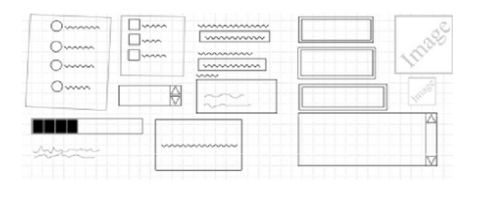
\includegraphics[width=0.75\textwidth]{Figura0302MediumFidelity}
    \caption{Ejemplo de un prototipo de fidelidad media.}
    \label{fig:MediumFidelity}
\end{figure}

	\item \textbf{High Fidelity}
	Son prototipos de una calidad m'as elevada, constan de un parecido mucho mayor a lo que se quiere representar, su detalle es mucho m'as alto por ende es m'as representativo. En la figura \ref{fig:HighFidelity} podemos apreciar un ejemplo de prototipo de  alto nivel de fidelidad.

\begin{figure}[ht]
    \centering
    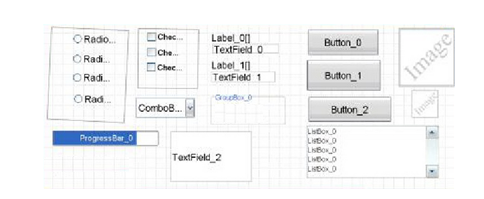
\includegraphics[width=0.75\textwidth]{Figura0303HighFidelity}
    \caption{Ejemplo de un prototipo de fidelidad alta.}
    \label{fig:HighFidelity}
\end{figure}	
\end{itemize}

El presente proyecto plantea realizar un sistema colaborativo para el dise\~no de interfaces de usuario mediante prototipos en alta fidelidad, de esta manera permitir a los usuarios ver el resultado m'as aproximado al resultado final. 
\chapter{Adaptaci'on}
\label{capitulocuatro}

\section{Adaptaci'on transparente y transformaci'on operacional}

Los sistemas groupware en tiempo real son construidos generalmente guiados por uno de los siguientes enfoques: conciencia de colaboración (collaboration awareness) y transparencia de colaboraci'on (collaboration transparency).
\medskip
Con el primer enfoque los groupware son desarrollados especialmente con el prop'osito de soportar la colaboraci'on y con mecanismos internos de conciencia de colaboraci'on desde su dise'no. Con el segundo enfoque, los groupware que est'an basados en sistemas existentes o nuevos, presentan mecanismos externos que no fueron pensados en el dise'no. [Qian Xia, 2006].
\medskip
Una ventaja de la colaboración transparente es que permite a los usuarios realizar colaboraciones con las aplicaciones que le son familiares, “¿Qui'en abandonaria su editor de texto favorito para usar una aplicaci'on de autoria colaborativa? - Who would abandon their favorite word processors to use a co-authorship application?” [Grudin, 1994 b], asimismo el agregar funcionalidades de colaboración en aplicaciones mono-usuario reduce el esfuerzo de desarrollar groupwares.

\section{Adaptaci'on Transparente}

A diferencia de otras t'ecnicas de transformaci'on de aplicaciones en aplicaciones compartidas, la adaptación transparente (TA) intenta transformar de forma transparente una aplicaci'on mono-usuario en una versión colaborativa del mismo, en el caso espec'ifico del proyecto, se trabaj'o 'unicamente con ambientes homog'eneos, lo cual significa que se requiere el uso de la misma aplicaci'on convertida en las sesiones de colaboraci'on.
\medskip
En los fundamentos de la adaptaci'on transparente, se trabaja con la API (Application Programming Interface - Interfaz de programaci'on de la aplicaci'on) para de esta manera interceptar las acciones realizadas por los usuarios y asi sin modificar el c'odigo
fuente de la aplicaci'on permitir la comunicaci'on del sistema mono usuario con los dem'as miembros de la sesi'on.
\medskip
El proyecto sobre el que se trabaj'o no cuenta con una API como tal, para poder realizar la intercepci'on de los eventos, pero tras analizar la estructura del proyecto, se identificaron las
operaciones claves a interceptar, es en este momento en el que se decidi'o usar herramientas de la Transformaci'on Operacional (OT) para manipular e interceptar los eventos generados, en este caso modificando levemente el manejo de los eventos dentro de la aplicaci'on de tipo mono usuario.

\medskip

El n'ucleo de la aplicaci'on de dise'no de interfaces se centra en tres acciones fundamentales:

\begin{itemize}
\item Agregar componente.
\item Editar componente.
\item Eliminar componente.
\end{itemize}

\medskip
Para poder llevar a cabo una adaptaci'on transparente como tal se pide poner especial 'enfasis en los siguientes puntos:
\medskip
\paragraph{Compatibilidad de la aplicaci'on​:}
Las caracter'isticas y funcionalidades de la interfaz de usuario as'i como los formatos de los documentos deben ser mantenidos.

\paragraph{Transparencia de la aplicaci'on:}
​No se deben realizar cambios al c'odigo original de la aplicaci'on en lo posible. Esta caracter'istica no pudo ser completada a falta de una forma de comunicaci'on con la aplicaci'on sobre la que se realiza el trabajo, por lo que se hizo 'enfasis en modificar lo m'inimo necesario para poder realizar la transformaci'on de la manera m'as transparente posible.

\paragraph{Respuesta local rapida:}
​La respuesta del sistema una vez modificado debe ser lo m'as parecida a la versi'on original. Para poder mantener esta caracter'istica puesto que como enfoque se escogi'o una arquitectura centralizada, se restringe que los miembros del equipo se encuentren de momento sobre la misma red.

\paragraph{Colaboraci'on sin restricciones:}
Los usuarios deben ser libres de realizar la mayor cantidad de operaciones con los datos en cualquier momento, lo que implica un
WYSIWIS (What you see is what I see - Lo que ves es lo que veo) relajado y trabajo concurrente. En un ambiente de WYSIWIS estricto, todos los integrantes del grupo de trabajo tienen que estar
estrictamente viendo lo mismo en un mismo ambiente. En cambio en un ambiente de WYSIWIS relajado si bien los integrantes se encuentran sobre un mismo sistema, presentan la libertad de moverse y realizar acciones diferentes a las de sus compa'neros de piso.

\paragraph{Conciencia de espacio de trabajo:}
​El sistema deberá soportar una variedad de
características de conciencia de espacio de trabajo, para permitir a los usuarios
conocer quien está trabajando con ellos y que están realizando.

\section{Modelo de adaptaci'on}

Para comenzar con la adaptación del sistema, se utilizo  el sistema para identificar las acciones fundamentales ya descritas, existen diferentes formas de realizar una misma acci'on dentro del sistema, y revisando la estructura de la forma en la que se manejan los eventos de los usuarios, se detect'o que una misma acci'on realizada desde diferentes lugares dentro de la aplicaci'on se traducen en diferentes acciones dentro de la misma \ref{fig:FV}, por lo que para comenzar con la transformaci'on del proyecto primero se dio paso a una ligera refactorizaci'on del sistema.

\begin{figure}[h]
    \centering
    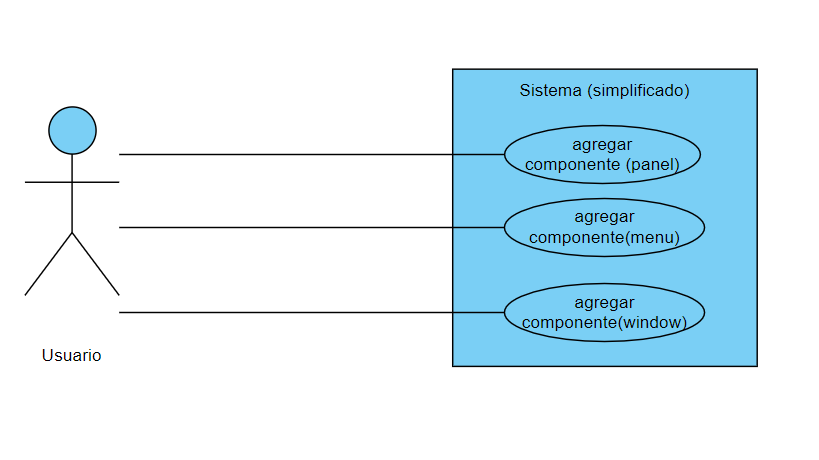
\includegraphics[width=0.55\textwidth]{Figura0401FirstView}
    \caption{Estado inicial del sistema, ejemplo.}
    \label{fig:FV}
\end{figure}




%
%\section{Motivaci'on}
%
%Para realizar el experimento se utiliz'o dos tipos de datos: contribuci'on a clases e interacci'on de clases; por las siguientes razones:
%
%\begin{itemize}
%\item \emph{Contribuciones a clases}. Cuando un conjunto de personas se reune para desarrollar software, tienden a trabajar juntos, por lo tanto la mayoria de las clases dentro de un proyecto son trabajadas por varias personas. Entender que personas trabajaron sobre ciertas clases, en ciertos periodos de tiempo ayuda a conocer el trabajo de cada contribuidor, que personas trabajaron en conjunto, que clases fueron modificadas en determinados tiempos, etc.\cite{Fritz}
%\item \emph{Interacci'on entre clases}. Al programar en el paradigma orientado a objetos, se hace uso de lo que es envio de mensajes o llamadas de m'etodos. Durante la ejecuci'on del programa, los objetos que son creados se mandan mensajes unos a otros. Entender entre que clases y en que momento se realiza este paso de mensajes ayuda a la optimizaci'on del software.\cite{Sillito}
%\end{itemize}
%
%\section{Conjunto de datos}
%
%Los dos conjuntos de datos utilizados para el experimento se escogieron a partir de las motivaciones anteriormente mencionadas, son datos reales del entorno de Pharo, recopilados en archivos .csv y se describen a continuaci'on:
%\begin{itemize}
%\item \emph{Contribuciones a clases}. Este conjunto de datos trata de las contribuciones realizadas sobre clases del modulo Trachel durante alg'un tiempo y los pesos representan la cantidad de l'ineas modificadas por un contribuidor en una clase. \\
%Trachel es un API (Application Programming Interface) de bajo nivel que permite dibujar elementos gr'aficos en Pharo, en la figura \ref{fig:Trachel} inciso a). se muestra el paquete de Trachel en el navegador de Pharo. Trachel esta compuesto por 5 elementos: contenedores gr'aficos (Canvas), figuras (Shape), eventos (Event), una entidad para enfocar porciones de contenedores (Camera) y ofrece animaci'on sobre figuras (Viva). \\
%Los datos est'an recopilados en el archivo Trachel.csv y se deduce que los datos fueron recopilados durante un periodo corto dado que s'olo se encuentra en el archivo 10 tiempos distintos. 'Este archivo contiene 525 tuplas en total, se distinguen a 22 contribuidores distintos y 98 clases del modulo Trachel.
%Por lo tanto en t'erminos de MultiPile Matrix el archivo Trachel.csv se representa en 10 matrices (tiempos) cada una de una tama'no de \textbar~22 x 98 \textbar.
%
%\begin{figure}[h]
%    \centering
%    \includegraphics[width=1\textwidth]{Figura0401Trachel}
%    \caption{En el inciso a). esta el paquete de Trachel y en el inciso b). algunas clases de Roassal ambos en el navegador de Pharo. Fuente: \url{http://pharo.org/}}
%    \label{fig:Trachel}
%\end{figure}
%
%\item \emph{Interacci'on entre clases}. Este conjunto de datos trata de como una clase del modulo de Roassal en tiempo de ejecuci'on interactua con otra, los pesos solo pueden ser dos valores 0 'o 1; es decir, tiene interacci'on o no. \\
%Roassal es el motor visual de Pharo, es utilizado para graficar elementos, en la figura \ref{fig:Trachel} inciso b). se muestra algunas de las clases de Roassal en el navegador de Pharo. Se desconoce el pedazo de c'odigo que se ejecuto para sacar los datos necesarios en el archivo resultante ClassDep04.csv. \\
%ClassDep04.csv contiene 643 tuplas en total, en 'este archivo se distinguen 19 tiempos distintos, con 26 clases distintas que mandan mensajes y 32 clases distintas que reciben mensajes.
%Por lo tanto en t'erminos de MultiPile Matrix el archivo ClassDep04.csv se muestra como 19 matrices (tiempos) cada una de una tama'no de \textbar~26 x 32 \textbar.
%\end{itemize}
%
%\section{Herramienta para comparar}
%Se opta por MS-Excel porque es una herramienta que se utiliza por defecto para manipular datos tabulares. Ofrece una larga lista de operaciones para manipular datos: filtros, ordenamiento, transformaciones, creaci'on de gr'aficos y definici'on de macros. Tambi'en excel tiene la ventaja de ser conocido por una gran poblaci'on y fue utilizado para muchos experimentos similares\cite{Cube14}.
%
%\section{Evaluaci'on}
%Esta evaluaci'on realiza una observaci'on sobre dos aspectos uno de ellos es el lenguaje, la primera es saber si el DSL es 'util; para ello se tiene la pregunta Q1 - ``?`Cu'an importantes son las caracter'isticas ofrecidas por MultiPile Matrix DSL para responder?''. El segundo aspecto es si esta visualizaci'on reduce el tiempo e incrementa la exactitud de las consultas, para ello se tiene la pregunta Q2 - ``?`Cu'an efectivo es MultiPile Matrix contra la herramienta est'andar?''.
%
%\section{Dise'no del experimento}
%Para realizar la evaluaci'on del proyecto se necesito de material, estrategia y participantes. El material que se dispuso para el experimento consiste de:
%\begin{itemize}
%\item \emph{Material de aprendizaje de Excel}: Este material de aprendizaje provee un imagen que resume las funciones que Excel ofrece para ordenar y filtrar. Para mayor informaci'on ver el anexo \ref{MaterialExcel}.
%\item \emph{Material de aprendizaje de MultiPile Matrix}: Se provee una descripci'on de las partes de MultiPile, las funcionalidades que ofrece acompa\~{n}adas de im'agenes. Es un resumen de la secci'on \ref{Aplicaciones}. Para mayor informaci'on ver el anexo \ref{MaterialMM}.
%\item \emph{Tarea 1}: Consiste en contestar con ayuda de alguna herramienta (MultiPile Matrix o Excel) a un cuestionario de 5 preguntas para el conjunto de datos referente a la contribuci'on de clases plasmado en el archivo Trachel.csv.
%\item \emph{Tarea 2}: Consiste en contestar con ayuda de alguna herramienta (MultiPile Matrix o Excel) a un cuestionario de 5 preguntas para el conjunto de datos referente a la interacci'on de clases plasmado en el archivo ClassDep04.csv.
%\item \emph{Retrospectiva}: Se pide la opini'on del participante de manera verbal para conocer la impresi'on que tuvo de la herramienta.
%\end{itemize}
%
%La estrategia consiste en la asignaci'on de las tareas entre los participantes, como se observa en la tabla \ref{tab:Tabla4.1}; tambi'en para que el ambiente sea lo m'as controlado posible, se realizo el experimento participante por participante en la misma maquina, de tal manera que se tienen 4 participantes para cada tarea con cada una de las herramientas.
%
%\begin{table}[h]
%\centering
%\begin{tabular}{l|l|l}
%\textbf{Participante} & \textbf{Tarea 1} & \textbf{Tarea 2} \\ \hline
%P1                    & EX               & MM               \\ \hline
%P2                    & MM               & EX               \\ \hline
%P3                    & EX               & MM               \\ \hline
%P4                    & MM               & EX               \\ \hline
%P5                    & EX               & MM               \\ \hline
%P6                    & MM               & EX               \\ \hline
%P7                    & EX               & MM               \\ \hline
%P8                    & MM               & EX               \\ \hline
%\end{tabular}
%\caption{Asignaci'on de herramientas y tareas. Fuente: Elaboraci'on propia}
%\label{tab:Tabla4.1}
%\end{table}
%
%A continuaci'on se describen las tareas que se crearon para el experimento. Para la Tarea 1 (Trachel.csv) se tienen las siguientes 5 preguntas: 
%\begin{itemize}
%\item Q1 - ?`Cu'al es la mayor cantidad de clases modificadas por un sola persona en un solo periodo entre los primeros cuatro periodos y quien fue?
%\item Q2 - ?`Qu'e contribuidores no realizaron cambios en clases del intervalo [2 - 8]?
%\item Q3 - ?`Qu'e clases fueron modificadas en cada tiempo durante todo el proyecto?
%\item Q4 - ?`Qu'e clases no fueron modificadas en el intervalo de tiempo donde TRArcShape fue modificado?
%\item Q5 - ?`Qu'e contribuidor no realizo cambios en el intervalo de tiempo donde TRCompositeShape fue modificado?
%\end{itemize}
%
%La 'unica pregunta que tiene como respuesta un dato es Q5, las dem'as son preguntas en las cuales se requiere identificar m'as de una clase o m'as de un contribuidor o m'as de un dato.
%
%Para la Tarea 2 (ClassDep04.csv) se tienen las siguientes preguntas:
%\begin{itemize}
%\item Q1 - ?`Qu'e clases no mandaron mensajes durante los 'ultimos cuatro tiempos?
%\item Q2 - ?`Qu'e par de clases (C1, C2, 1) interactuan en cada tiempo que pertenece al intervalo [1 - 3]?
%\item Q3 - ?`Qu'e clases reciben mensajes solo en el ultimo tiempo?
%\item Q4 - ?`Qu'e clases reciben mensajes en cada tiempo en el intervalo donde RTMapExample mando o recibio mensajes?
%\item Q5 - ?`Qu'e clases no mandaron mensajes en el intervalo donde RTPopup mando o recibio mensajes?
%\end{itemize}
%
%Para todas las preguntas se requiere identificar un conjunto de clases o pares de clases.
%
%\section{Modo de calificaci'on}
%\label{sec:cali}
%Un participante puede responder a las preguntas con las respuestas que crea correctas. Este experimento se basa en la puntuaci'on de F-Measure o Valor-F, esta medida es una combinaci'on de la precisi'on y el recall. Para cada pregunta se calific'o de la siguiente forma: 
%\begin{itemize}
%\item \emph{Precisi'on}. Est'a dada por la cantidad de respuestas correctas relacionadas divido entre la cantidad de respuestas seleccionadas; es decir: $RCS/RS$.
%\item \emph{Recall}. Est'a dado por la cantidad de respuestas correctas relacionadas divido entre la cantidad de respuestas correctas; es decir: $RCS/RC$.
%\end{itemize}
%La puntuaci'on para cada pregunta se encuentra entre 0 y 1.
%Para cada tarea se tiene en cuenta la precisi'on y el recall, la nota de un participante en recall $x$ est'a dada por: \\* $PR(x) = \sum_{n=1}^5 PuntuacionRecall(Q_n, x)$ y en precisi'on por:
%\\* $PP(x) = \sum_{n=1}^5 PuntuacionPrecision(Q_n, x)$. Ambas puntuaciones se encuentran entre 0 y 5. Siendo 5 la mayor puntuaci'on posible.
%
%El F-Measure de cada participante esta dado por $P(x) = 2 * (PP(x) * PR(x)) / (PP(x) + PR(x))$. Tambi'en 'esta puntuaci'on se encuentra entre 0 y 5.
%
%\section{Estudio piloto}
%Antes de realizar todo el experimento, se realizo un estudio piloto con dos personas de la Universidad de Santiago de Chile, ambos finalizan estudios de maestria en ciencias de la computaci'on. Tambi'en ambos conocen Pharo y manejan Excel durante m'as de 5 a'nos. Este estudio ayudo a observar algunos puntos del experimento como:
%
%\begin{itemize}
%\item Ambas tareas se pueden realizar con Excel y MultiPile Matrix.
%\item Ambos participantes tuvieron la necesidad de observar documentaci'on sobre Excel. Se opto como conveniente que los participantes recurran a busquedas en internet sobre Excel como ayuda para el experimento.
%\item El material de aprendizaje de MultiPile Matrix se modifico con algunas observaciones de parte de los participantes de piloto.
%\item El cuestionario original tenia preguntas ambiguas o no claras, entonces se analizo y mejoro el cuestionario. 
%\end{itemize}
%
%El anexo \ref{MaterialMM} ofrece mayor informaci'on del estudio piloto.  
%
%\section{Resultados}
%Se realizo el experimento con 8 participantes de los cuales se puede destacar las siguientes caracter'isticas: todos tenian experiencia de minimamente 4 a'nos con Excel, todos conocian el paradigma OO y programaron en 'el, pero ninguno tenia conocimiento de Pharo. Entre estos participantes se encuentran 3 profesionales en ingenier'ia inform'atica, 3 estudiantes no graduados realizando su tesis en ingenier'ia inform'atica o de sistemas y 2 estudiantes no graduados entre sexto semestre y noveno semestre de las carreras de ingenier'ia inform'atica o de sistemas.
%
%\begin{figure}[h]
%    \centering
%    \includegraphics[width=0.55\textwidth]{Figura0402RE}
%    \caption{Resultado de la precisi'on y recall del experimento y las puntuaciones de Excel resaltadas con gris. Fuente: Elaboraci'on propia}
%    \label{fig:RE}
%\end{figure}
%
%En la figura \ref{fig:RE} se muestran los resultados de precisi'on y recall de cada participante, la primera columna tiene los identificadores de los participantes. Las siguientes 10 columnas muestran la puntuaci'on para cada pregunta de la tarea 1 y luego de la tarea 2.
%
%Las 'ultimas dos columnas son la puntuaci'on total mencionada en la secci'on \ref{sec:cali} para Excel y MultiPile Matrix. Las puntuaciones para Excel estan resaltadas en gris para una lectura m'as comprensible. 
%
%\begin{figure}[h]
%    \centering
%    \includegraphics[width=0.75\textwidth]{Figura0403RT}
%    \caption{Resultado del Valor-F de cada participante en el experimento y en la parte izquierda los tiempos que se demor'o cada participante. Fuente: Elaboraci'on propia}
%    \label{fig:RT}
%\end{figure}
%
%Mientras que en la figura \ref{fig:RT} la tabla de la parte derecha muestra las puntuaciones de cada participante del Valor-F, criterio en el que este experimento se basa. Y en la tabla izquierda se presenta el tiempo que tardo cada participante al realizar la tarea 1 y la tarea 2, este tiempo esta en minutos. Nuevamente las puntuaciones para Excel estan resaltadas en gris. 
%
%\begin{figure}[h]
%    \centering
%    \includegraphics[width=0.4\textwidth]{Figura0404Box}
%    \caption{Resultado del an'alisis del Valor-F. Fuente: Elaboraci'on propia}
%    \label{fig:Box}
%\end{figure}
%
%Para el an'alisis de los resultados se realizo la figura \ref{fig:Box} que a simple vista muestra que MultiPile Matrix tiene un efecto positivo tanto en precision como en recall. En la misma figura se muestra el an'alisis de los resultados de Valor-F, en la cual MultiPile Matrix sigue manteniendo un efecto positivo, con una m'axima puntuaci'on de 5, una m'inima de 4.5 y la media de $4.875 \pm 0.0590$, mientras que con Excel una m'axima de 4.6, una m'inima de 1.78 y la media de $3.448 \pm 0.2863$. 
%
%Para demostrar que los resultados no son a favor de la herramienta por suerte, se realizaron los siguientes pasos:
%
%\begin{itemize}
%\item El primer paso es formular una hipotesis nula, en este caso la hipotesis nula es: La puntuaci'on de MultiPile Matrix no es diferente a la de Excel. 
%\item El segundo paso es tratar de rechazar la hipotesis nula. Para rechazarla se realiza primero un test de normalidad, en este caso se uso ``Shapiro-Wilk normality test'' \cite{test}, 'este test verifica si los resultados son parte de una poblaci'on distribuida normalmente; este test tiene condiciones sobre los valores para ser considerado una opci'on para rechazar la hipotesis nula. Debido a la cantidad de datos y a su valor se encuentra que los datos de MultiPile Matrix no son normales y esa es una condici'on para continuar con este test.
%\item Ya que los datos no son normales se utilizo ``Mann-Whitney test'' \cite{test}, 'este test trabaja con valores no normales e indica si hay una diferencia significativa entre los resultados de Excel y MultiPile Matrix. Se considera que hay una diferencia significativa o que la hipotesis nula es rechazada, cuando el valor $P$ del calculo del test es menor a 0.05.
%\end{itemize}
%
%Una vez realizado el ``Mann-Whitney test''($P<0.05$) teniendo un $P = 0.0005$, que indica que la diferencia entre los resultados de Excel y MultiPile Matrix es significativa.
%
%Por lo tanto en este experimento se aprecia que:
%\begin{itemize}
%\item Los participantes consiguieron puntuaciones mejores y significativas usando MultiPile Matrix que con Excel.
%\item Los participantes completaron el cuestionario mucho m'as r'apido usando MultiPile Matrix que con Excel.
%\end{itemize}
%
%\section{Uso de Excel}
%Se observo a cada participante a medida que respondia las preguntas con Excel, 3 participantes recurrieron a ayuda online acerca de las funciones para quedarse con datos 'unicos, 5 participantes usaron distintas funciones de Excel, por ejemplo la funci'on COUNTIF, SUMIF, o agregando columnas extras, teniendo as'i un mejor tiempo que los dem'as participantes. 
%Se debe resaltar que no existe alguna pregunta en la que todos los participantes tuvieran el puntaje m'aximo. Y que el participante P8 fue el que mejor nota obtuvo, pero solo utilizo funciones de ordenamiento, filtros y filtros 'unicos.
%
%\section{Uso de MultiPile Matrix}
%Al observar los usos de MultiPile Matrix, fue sorprendente notar que no utilizaron todas las caracter'isticas del material de aprendizaje. Si bien en las primeras preguntas de ambas tareas se debia realizar una apilaci'on de un intervalo, los participantes P2 y P3 solo vieron necesario ver el timeLine para responder. Los participantes P5 y P4 a medida que realizaban una apilaci'on por criterio tambi'en resaltaban las relaciones que satisfacian el mismo criterio. Para la Q2 de la tarea 2 todos los participantes utilizaron el resaltado de peso, obteniendo respuestas correctas con MultiPile Matrix. Para la tarea 1, las preguntas Q2, Q3 y Q5 tuvieron respuestas correctas para todos los participantes, utilizando las opciones de apilaci'on y observando las partes que componen una pila. Para la tarea 2, las preguntas Q1, Q2, Q4 y Q5 tuvieron respuestas correctas para todos los participantes, utilizando resaltado y opciones de apilaci'on.
%
%\section{Retrospectiva}
%Despu'es del experimento, se cuestion'o a cada participante acerca de las tareas realizadas. Sus respuestas a los cuestionarios no fueron calificadas ese mismo momento, para que no se sientan presionados al responder.
%
%Mientras usaron MultiPile Matrix los participantes P5 y P8 sintieron que la navegaci'on entre barras verticales era algo complicado, sin embargo ambos tienen una buena puntuaci'on. Ningun participante sinti'o que las preguntas fueran inadeacuadas, pues cada tarea se podia responder con cualquiera de las dos herramientas. Tambi'en las preguntas fueron percibidas como representativas como tareas que alguna vez un desarrollador puede llegar a afrontar. Todos los participantes sintieron preferencia a MultiPile Matrix, el participante P6 estuvo interesado en MultiPile Matrix por el aspecto de seguimiento a equipos de desarrollo, con este participante se hablo sobre GitHub y que podria ofrecer como mejora MultiPile Matrix. El participante m'as emocionado fue P8 por la posibilidad de que otras cosas se podria visualizar y analizar, se sinti'o atraido por la idea y el dise'no de la visualizaci'on.
%
 

\addcontentsline{toc}{chapter}{Bibliograf'ia}
\chapter*{Bibliograf'ia}
\bibliography{013-Bibliografia-Bibliografia}
\end{document}